\documentclass[12pt]{report}

\usepackage[letterpaper, hmargin=0.75in, vmargin=0.75in]{geometry}

\usepackage{
    courier,
    algorithm,
    algpseudocode,
    listings,
    underscore,
    authblk,
    hyperref,
    tikz,
    tabularx,
    float,
    graphicx,
	 color
}

\lstset{basicstyle=\footnotesize\ttfamily}

\setlength{\parindent}{0pt}

\begin{document}

\title{RTX Software Design Report}

\author{
    Clement Hoang\\
		20531116\\
    \texttt{c8hoang@uwaterloo.ca}
    \and
    David Su\\
		20516776\\
    \texttt{dysu@uwaterloo.ca}
    \and
    Cole Vander Veen\\
		20503626\\
    \texttt{cgvander@waterloo.ca}
    \and
    Peter Li\\
		XXXXXXXXX\\
    \texttt{y648li@uwaterloo.ca}
}

\date{Winter 2016}

\maketitle


\tableofcontents
\listofalgorithms
\listoffigures

\chapter{Introduction}

The purpose of this report is to outline the design of the RTX written by the group members, Clement Hoang, David Su, Peter Li, and Cole Vander Veen, as part of the SE350 course at the University of Waterloo. The OS is designed for a Keil MCB1700 Cortex-M3 board, with a LPC1768 microcontroller.

It is aimed to provide documentation for the operating system, in order to facilitate the use and understanding for anyone interested in programming for the OS. As such, this report outlines the global variables used in the OS, and then moves on to describing the kernel API in a modular and chronological way, from when we implemented it. Finally, the report closes with some analysis on the OS, and challenges that the group faced for the duration of the lab.

\chapter{Design Description}

\section{Global Variables and Data Structures}
\begin{itemize}
  \item \texttt{memQueue}: A data structure that models the free physical memory in the OS, by splitting the heap into blocks of equal size. It is represented by a \texttt{MemQueue} data structure, which is a linked list of \texttt{MemBlock} nodes of size \texttt{BLOCK_SIZE}. It is used by the kernel API when releasing and requesting memory, by popping a block when it is used by a process, and pushing it back in when it is released.
    \begin{itemize}
      \item \texttt{MemBlock}: To expand, the \texttt{MemBlock} is a C-struct that holds a pointer to the next \texttt{MemBlock} in the queue. It also has reserved space in the front in case the block needs to hold an envelope.
    \end{itemize}
  \item \texttt{gp_pcbs}: A pointer to an array of \texttt{PCB} structs. It holds the state of all the process control blocks that are in the OS, and is interacted with by functions that change and read PCB states. For example, setting the process priority or getting the process priority uses \texttt{gp_pcbs} to access the priority of a specific PCB.
    \begin{itemize}
      \item \texttt{PCB}: a model of a process and its state. The \texttt{PCB} contains the following fields:
        \begin{itemize}
          \item \texttt{mp_sp}: stack pointer of the process
          \item \texttt{m_pid}: ID of the process
          \item \texttt{m_priority}: priority of the process
          \item \texttt{m_state}: state of the process
          \item \texttt{nextPCB}: pointer to the next \texttt{PCB}, if it is in a queue
          \item \texttt{msgHead}: beginning of the message queue
          \item \texttt{msgTail}: end of the message queue
        \end{itemize}
    \end{itemize}
  \item \texttt{gp_stack}: 
  \item \texttt{p_end}
  \item \texttt{numOfBlocks}
\end{itemize}

\section{Memory Management}

\subsection{Memory Structure}

dsfdasfdsafdsafdsafsadfdsaf

\begin{figure}
	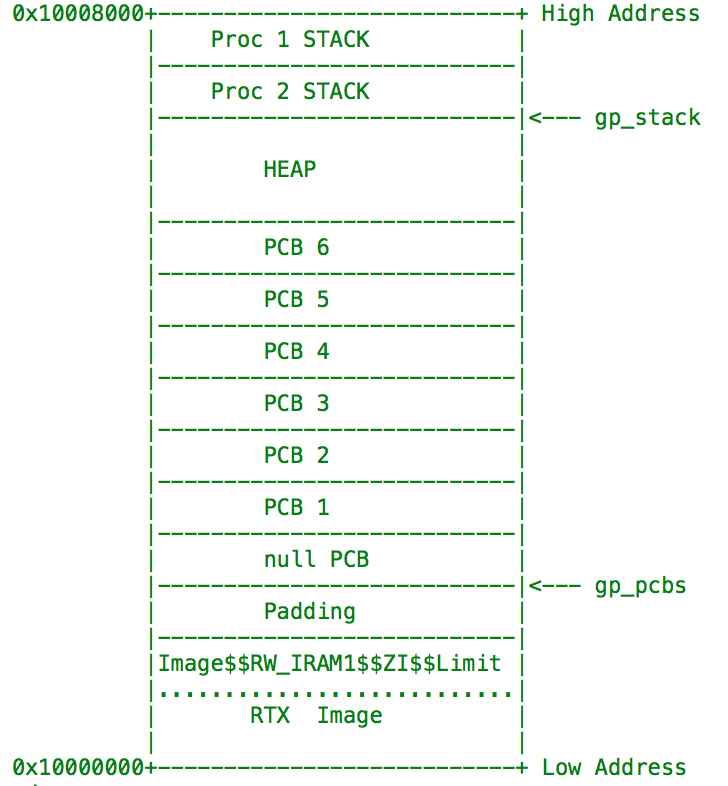
\includegraphics{memory.png}
\caption{Memory Layout}

\end{figure}

\subsection{Requesting Memory Blocks}

\begin{minipage}{\textwidth}
\begin{lstlisting}[language=C, frame=single]
int k_request_memory_block(void);
\end{lstlisting}
\end{minipage}

describe input, output, effects

\begin{algorithm}
  \caption{k_request_memory_block}
  \begin{algorithmic}[1]
    \Procedure{request\_memory\_block}{}
      \While{heap is full}
			\State {block the current process}
	  \EndWhile
	  \State {update the free space list}
	  \State {return the address of the top of the block}
    \EndProcedure
  \end{algorithmic}
\end{algorithm}

\subsection{Releasing Memory Blocks}

\begin{minipage}{\textwidth}
\begin{lstlisting}[language=C, frame=single]
int k_release_memory_block(void* memory_block);
\end{lstlisting}
\end{minipage}

describe input, output, effects

\begin{algorithm}
  \caption{The memory release function}
  \begin{algorithmic}[1]
    \Procedure{release\_memory\_block}{*memory_block}
      \If{this block is the top block of the heap}
			\State {modify heap header node (never gets overwritten)}
	  \EndIf
	  \If{there is free space immediately beneath this block}
			\State {combine them by increasing this block's length}
	  \Else { this block becomes a new block node, is added to the list}
	  \EndIf
	  \If{there is free space immediately beneath this block}
			\State {combine them by increasing this block's length}
	  \EndIf
	  \If{a process is blocked on memory}
			\State {unblock that process, release the processor}
	  \EndIf
    \EndProcedure
  \end{algorithmic}
\end{algorithm}

\pagebreak


%%%%%%%%%%%%%%%%%%%%%%%%%%%%%%%%%%%%%%%%%%%%%%%%%%%%%%%%%%%%%

\section{Processor Management}

\subsection{Process Control Structures}
DFASFAFD

\subsection{Process Queues}

fsadfasdfadsf

\subsection{Process Scheduling}
sdfasdfasdfdasf

%%%%%%%%%%%%%%%%%%%%%%%%%%%%%%%%%%%%%%%%%%%%%%%%%%%%%%%%%%%%%

\section{Process Priority Management}

\subsection{Get Process Priority}

asdfadsfasf

\subsection{Set Process Priority}

dsfasdfasfsfdf

%%%%%%%%%%%%%%%%%%%%%%%%%%%%%%%%%%%%%%%%%%%%%%%%%%%%%%%%%%%%%

\section{Interprocess Communication}

\subsection{Message Structure}

dsfadsfadsfdasfdafs

\subsection{Sending Messages}

adsfdsafasdfasf

\subsection{Receiving Messages}

dsfafasfdasf

\subsection{Delayed Send}


sdfasfasfd

%%%%%%%%%%%%%%%%%%%%%%%%%%%%%%%%%%%%%%%%%%%%%%%%%%%%%%%%%%%%%

\section{Interrupts and I-Processes}

\subsection{UART I-Process}

The UART interrupt is enabled to send output to a display, and to receive input from the user. The OS handles those interrupts by registering a \texttt{UART0_IRQHandler} function that will be called whenever a UART interrupt occurs. 

The file \texttt{uart_irq.c} is initialized by calling the function \texttt{uart_irq_init}. This function initializes the UART interrupts by setting the appropriate flags and choosing the correct UART port. 

Below is the interrupt handling pseudocode, starting with UART0_IRQHandler:
\begin{algorithmic}[1]
  \Function{UART0_IRQHandler}{}
    \State push registers onto stack
    \State call c_UART0_IRQHandler_wrapper()
    \State pop registers off stack
  \EndFunction
\end{algorithmic}
\begin{algorithmic}[1]
  \Function{c_UART0_IRQHandler_wrapper}{}
    \State call c_UART0_IRQHandler()
    \If{there is another ready process with higher priority than the current process}
      \State call k_release_processor()
    \EndIf
  \EndFunction  
\end{algorithmic}
\begin{algorithmic}[1]
  \Function{c_UART0_IRQHandler}{}
    \If{receive data available}
      \State g_char_in = newly received char
      \If{g_char_in == null character} 
        \State\Return
      \EndIf

      \State echoMsg = get memory block (non blocking)
      \If{echoMsg is not null}
        \State echoMsg-$>$mtype = ECHO
        \If{g_char_in == '\textbackslash r'}
          \State echoMsg-$>$mtext = \verb|"\n\r\0"|
        \Else
          \State echoMsg-$>$mtext = g_char_in + \verb|'\0'| 
        \EndIf
        \State send echoMsg (no preemption) to KCD
      \EndIf
      \If{cur_msg is null}
        \State cur_msg = get memory block (non blocking)
        \If{cur_msg is null (no more memory)}
          \State\Return
        \EndIf

        \State msg_str_index = 0
      \EndIf

      \If{g_char_in == '\textbackslash r' or message about to overflow memory block}
        \State cur_msg-$>$mtext += '\textbackslash 0'
        \State cur_msg-$>$mtype = DEFAULT
        \State send cur_msg (no preemption) to KCD
        \State reset cur_msg, msg_str_index
      \Else
        \State cur_msg-$>$mtext += g_char_in
      \EndIf
    \ElsIf{transmit interrupt enabled}
      \If{*gp_buffer != null character}
        \State send *gp_buffer
        \State gp_buffer = next location in circular buffer
      \Else
        \State disable transmit interrupt
        \State send null character
        \State reset gp_buffer and g_buffer_end
      \EndIf
    \EndIf
  \EndFunction
\end{algorithmic}

If there is an incoming character, immediately forward it to the KCD (assuming there is free memory) to echo back to the user. Also, add that character to a buffer. Once a newline is encountered, send the entire buffer to the KCD to decode

If there are still messages in the transmit buffer, send the next character. If the character is a null character, disable the transmit interrupt as the transmission is finished. 


Also, there is an \texttt{enable_UART_transmit()} function that sets the appropriate flags to enable the interrupt for outputting characters. This function is called by the CRT to begin outputting characters.


\subsection{Timer I-Process}

sdfasfdafd

%%%%%%%%%%%%%%%%%%%%%%%%%%%%%%%%%%%%%%%%%%%%%%%%%%%%%%%%%%%%

\section{System Processes}

\subsection{Null Process}

sdfdasfafadsf

\subsection{CRT Process}

The CRT's sole responsibility is to output the contents of the messages they receive to the UART.

\begin{algorithmic}[1]
  \Function{crtProc}{}
    \While{true}
      \State msg = receive\_message()
      \State copy msg-$>$mtext to output buffer
      \State enable\_UART\_transmit() 
      \State release\_memory\_block(msg)
    \EndWhile
  \EndFunction
\end{algorithmic}

\begin{algorithmic}[1]
  \Function{copyToBuffer}{str}
    \For{each char in str}
      \State g_buffer[g_buffer_end] = char
      \State g_buffer_end = (g_buffer_end + 1) mod BUFFER_SIZE
    \EndFor
  \EndFunction
\end{algorithmic}

\subsection{KCD Process}

The KCD's (Keyboard Command Decoder) responsibility is to decode messages that it receives, and forward them to the appropriate process that has registered itself to handle these types of messages. 

\begin{algorithmic}[1]
  \Function{kcdProc}{}
    \State identifiers = empty array
    \State processes = empty array
    \State numIdentifiers = 0
    \While{true}
      \State msg = receive\_message()
      \If{msg-$>$mtype == KCD\_REG}
        \State add msg's identifier to identifiers
        \State add msg's sender to processes
        \State numIdentifiers++
        \State release\_message\_block(msg)
      \ElsIf{msg-$>$mtype == ECHO}
        \State send\_message(PID\_CRT, msg)
      \Else
        \If{msg-$>$mtext starts with '\%'}
          \State handler = search for handler in identifiers
        \EndIf
        \If{no handler for this type of message}
          \State release\_memory\_block(msg)
        \Else
          \State send\_message(handler, msg)
        \EndIf

        \If{msg-$>$mtext begins with '!'}
          \State search through PCBs for processes in ready state
          \State debugMsg = create message with those processes
          \State send\_message(PID\_CRT, debugMsg)
        \ElsIf{msg-$>$mtext begins with '@'}
          \State search through PCBs for processes in blocked state
          \State debugMsg = create message with those processes
          \State send\_message(PID\_CRT, debugMsg)
        \ElsIf{msg-$>$mtext begins with '\#'}
          \State search through PCBs for processes in blocked on message state
          \State debugMsg = create message with those processes
          \State send\_message(PID\_CRT, debugMsg)
        \EndIf
      \EndIf
    \EndWhile 
  \EndFunction
\end{algorithmic}

This processes repeatedly receives messages. If it is a keyboard command registration, the process saves the identifier along with the process that is registered to handle those commands. If it is an echo command, the message is merely forwarded to the CRT. Otherwise, if the message is an actual command (i.e. it starts with a '\%'), the message is forwarded to the process that is registered to handle it, if it exists. Finally, if the message begins with any debug hotkey, the corresponding debug output is sent to the CRT.

%%%%%%%%%%%%%%%%%%%%%%%%%%%%%%%%%%%%%%%%%%%%%%%%%%%%%%%%%%%%%

\section{User Processes}

\subsection{Wall Clock Process}

This process receives messages to reset, start at a specified time, and stop the wall clock. Once started, the clock will print the elapsed time every second.

\begin{algorithmic}[1]
  \Function{wallClockProc}{}
    \State register itself with KCD to handle '\%W' commands
    \State id = 0
    \While{true}
      \State msg = receive\_message()
      \If{msg contains reset command}
        \State id++
        \State time = 0
        \State send increment time command to itself, delayed 1 second
        \State construct time string, send to CRT to print
      \ElsIf{msg contains increment command}
        \If{msg's id == id}
          \State time++
          \State send increment time command to itself, delayed 1 second
          \State construct time string, send to CRT to print
        \Else
          \State release\_memory\_block(msg)
        \EndIf
      \ElsIf{msg contains a start at specified time command}
        \State id++
        \State time = parseTime(msg)
        \State send increment time command to itself, delayed 1 second
        \State construct time string, send to CRT to print
      \ElsIf{msg contains stop command}
        \State id++
        \State release\_memory\_block(msg)
      \Else
        \State release\_memory\_block(msg)
      \EndIf
    \EndWhile
  \EndFunction  
\end{algorithmic}

\subsection{Set Priority Process}

dsfasdfasdfadsf

\subsection{Stress Test Processes}

dfdasfasdfads

\section{Initialization}

dasfasfasfd

\section{Testing}

dfadsfasdf

\section{Major Design Changes}

dsfdafadsf

\chapter{Lessons Learned}

\section{Source Control and Code Management}

sdfdsafsadf

\chapter{Team Dynamics and Individual Responsibilities}

\section{adsfadsf}

dfasfasdf

\chapter{Timing Analysis}

\end{document}
